\section{Results}
\label{sec:results}
\subsection{Contract and operational boundaries}
All 22 selected counterexample tests pass when replayed individually on the same retained executable as the context diagnostic. Each invocation reports one passed test, zero failed tests, and zero ignored tests; none times out. Executable hashes match before and after every invocation, and the 774-path source manifest, all 1003 archived source files, and the primary raw report remain unchanged. Table~\ref{tab:counterexamples} groups the tested boundaries.

\begin{table}[t]
\small
\caption{Selected counterexamples replayed on the retained executable. Each test is executed once. Counts indicate successful expected behavior, not sampled failure-detection accuracy.}
\label{tab:counterexamples}
\begin{tabularx}{\columnwidth}{@{}Xr@{}}
\toprule
Boundary and tested distinction & Passed\\
\midrule
Acceptance: revision, receipt, authority, and approval conditions & 11/11\\
Producer conflict: applicable failures survive another producer's pass & 2/2\\
Dependency ownership: uncertain mappings remain qualified & 2/2\\
Scope and observability: unresolved work and verification state & 2/2\\
Evaluator: grading behavior on constructed counterexamples & 5/5\\
\midrule
Total & 22/22\\
\bottomrule
\end{tabularx}
\end{table}

These tests give concrete instances of the contract in Section~\ref{sec:contract}: a result with the wrong revision or authority cannot supply the required support, and a passing record from another producer does not remove an applicable blocking failure. The outcomes validate the selected assertions under the tested fixtures. They do not establish the adequacy of arbitrary verification plans or resistance to adaptive attacks. Earlier executions of these tests used a different build; the replay resolves that provenance difference without pooling the two executions.

All eleven primary controls pass. In the competing-write control, two operations begin with the same observed hash; one commits and one is rejected. The read-only and workspace-boundary controls reject their ineligible operations. Partial-graph reporting retains its incomplete status. Under syntax-cache pressure, the recorded run performs 13,168 trims and still reports 96 files, 96 matches, zero failures, and complete coverage. Workspace-relative verification singleflight passes its targeted duplicate-execution check.

These controls support RQ1 at their stated granularity. For example, the concurrent-write outcome is evidence for the guarded single-file path under the tested schedule. It does not establish transactional multi-file editing or coordination with every external process.

\subsection{Bounded source delivery}
For every budget--phase condition, identity, complete original-body delivery, and current file-metadata SHA each satisfy all 686 annotated obligations. All 406 eligible editing attempts satisfy the strict edit-input predicate. Across six conditions, this corresponds to 4116 required source instances and 2436 eligible editing attempts. There are no query errors, response-budget overruns, or warm-up errors.

These saturated outcomes answer RQ2 for the retained corpus. They also reveal the corpus's limited discrimination: its required source is small enough to fit even the lowest budget. A 100\% source score therefore says little about how additional budget changes other useful evidence. Figure~\ref{fig:budget} juxtaposes the saturated delivery measures with decision-record exposure and actual response size to make that distinction visible.

\begin{figure*}[t]
\centering
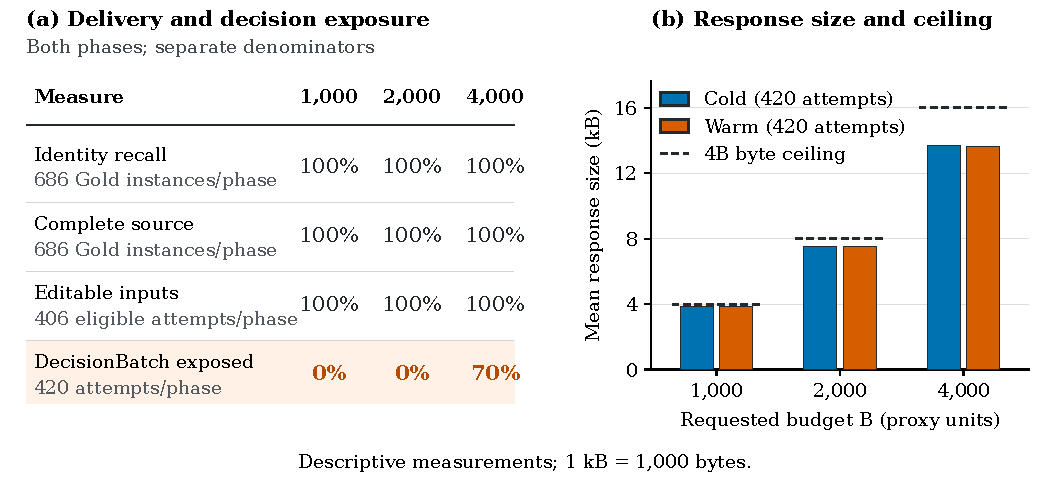
\includegraphics[width=\textwidth]{figures/budget_exposure.pdf}
\caption{Budget changes different outputs differently. Left: source delivery, editable-input success, and serialized decision-record exposure use distinct denominators (686 source obligations, 406 editable attempts, and 420 total attempts per condition). Rates agree between cold and warm phases; phases are not pooled. Right: mean serialized response bytes remain below the $4B$ ceiling implied by the accounting rule. The lowest budget already saturates the source-delivery measures.}
\label{fig:budget}
\end{figure*}

\subsection{Nested readiness predicates}
For RQ3, the attempt-level identity, body, and body-plus-file-metadata predicates each classify 413 answerable observations as positive per condition. The full editable-input predicate classifies 406. Omitting write eligibility therefore admits seven read-only observations, or $7/413=1.69\%$ of answerable observations. Across all six conditions, the 42 affected observations repeat the same read-only fixture; they are not 42 independently discovered vulnerabilities.

The result is small but diagnostic. Correct localization, original source, and fresh hashes can all be present while editing remains inadmissible. Removing the extra file-metadata SHA predicate produces no further separation in this corpus; the preceding body predicate already checks the source-window hash. The analysis therefore does not identify independent causal effects for each nested condition. It establishes a concrete counterexample to equating source availability with edit readiness.

\subsection{Budget, visibility, and latency}
Serialized \code{DecisionBatch} exposure is 0/420 at budgets 1000 and 2000, and 294/420 (70\%) at budget 4000, in both phases. Thus, equal source recall does not imply equal visibility into the runtime's structured decisions. This finding answers the visibility part of RQ4 without interpreting the exposed records as correct decisions on real tasks.

\begin{table*}[t]
\centering\small
\caption{Descriptive cost of the frozen primary run. Each row contains 420 measured calls. Latency quantiles summarize calls; the ECDF in Figure~\ref{fig:latency} uses scenario medians instead. Bytes are serialized JSON bytes, not model tokens.}
\label{tab:cost}
\begin{tabular}{@{}rrcrrrr@{}}
\toprule
Budget $B$ & Byte ceiling $4B$ & Phase & Mean bytes & p50 (ms) & p95 (ms) & Decision exposure\\
\midrule
1000 & 4000 & Cold & 3850.14 & 40.186 & 70.913 & 0/420\\
1000 & 4000 & Warm & 3849.71 & 27.030 & 51.216 & 0/420\\
2000 & 8000 & Cold & 7506.04 & 34.795 & 61.286 & 0/420\\
2000 & 8000 & Warm & 7503.97 & 20.738 & 34.736 & 0/420\\
4000 & 16000 & Cold & 13667.22 & 25.709 & 56.378 & 294/420\\
4000 & 16000 & Warm & 13663.93 & 12.948 & 25.150 & 294/420\\
\bottomrule
\end{tabular}
\end{table*}

\begin{figure}[t]
\centering
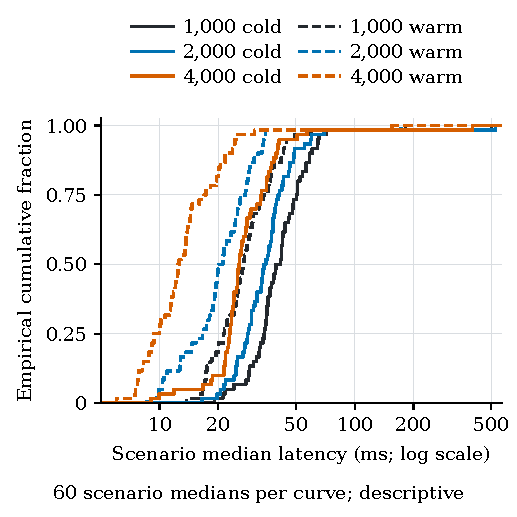
\includegraphics[width=\columnwidth]{figures/latency_ecdf.pdf}
\caption{Latency distributions of scenario medians, with a logarithmic latency axis. Each of the six curves contains 60 medians of seven repeated calls. Color denotes budget and line style denotes harness phase. All observed medians, including the upper tail, are retained.}
\label{fig:latency}
\end{figure}

Across the six conditions, median call latency ranges from 12.948 to 40.186\,ms; the largest p95 is 70.913\,ms. Warm-phase summaries are lower than their corresponding cold-phase summaries. Larger budgets also have lower measured latency in this run. The latter relationship is not a demonstrated speedup caused by budget: fixed budget order, packing work, shared operating-system caches, and uncontrolled host load are potential confounders. The defensible conclusion is that the call medians and 95th percentiles were in the tens of milliseconds on this host, under the stated debug-build protocol; individual observations and some scenario medians have a longer tail.

The combined result is a three-way separation. Source obligations can be completely delivered, an edit can still be ineligible, and structured decision records can still be absent. Treating any one of these measurements as a universal readiness score would hide an observable difference in the returned interface.
